\begin{figure}[h]
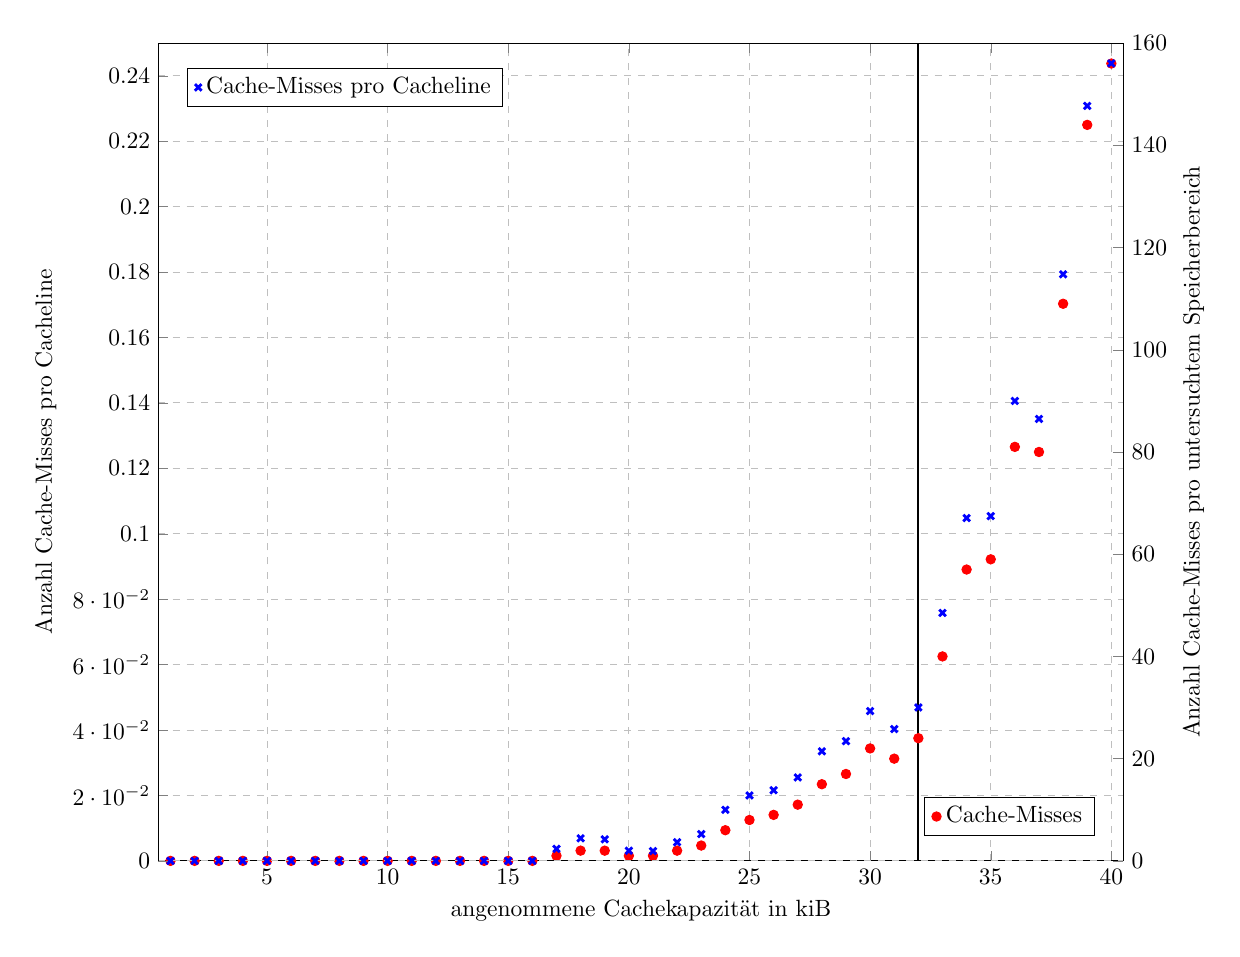
\begin{tikzpicture}[scale=0.85]

\pgfplotsset{
    width=16cm,
    xmin=0.5,
    xmax=40.5,
    xlabel=angenommene Cachekapazität in $\textrm{kiB}$,
    grid style=dashed,
    xmajorgrids=true,
    xminorgrids=true
}

\begin{axis}[
  axis y line*=right,
  ymin=0, ymax=160,
  ylabel=Anzahl Cache-Misses pro untersuchtem Speicherbereich,
  legend pos=south east,
]

\addplot[mark=*,red,only marks]
    coordinates {
    (1,0 ) (2,0 ) (3,0 ) (4,0 ) (5,0 ) (6,0 ) (7,0 ) (8,0 ) (9,0 )
    (10,0 )(11,0 )(12,0 )(13,0 )(14,0 )(15,0 )(16,0 )(17,1 )(18,2 )(19,2)
    (20,1 )(21,1 )(22,2 )(23,3 )(24,6 )(25,8 )(26,9 )(27,11)(28,15)(29,17)
    (30,22)(31,20)(32,24)(33,40)(34,57)(35,59)(36,81)(37,80)(38,109)(39,144)(40,156)
    };\legend{Cache-Misses}

\addplot +[thick,mark=none,black] coordinates {(32, 0) (32, 160)};

\end{axis}

\begin{axis}[
  axis y line*=left,
  axis x line=none,
  ymin=0, ymax=0.25,
  ylabel=Anzahl Cache-Misses pro Cacheline ,
  legend pos=north west,
  ymajorgrids=true,
  yminorgrids=true
]

\addplot[very thick,mark=x,blue,only marks]
  coordinates{
    (1,0 ) (2,0 ) (3,0 ) (4,0 ) (5,0 ) (6,0 ) (7,0 ) (8,0 ) (9,0 )
    (10,0 )(11,0 )(12,0 )(13,0 )(14,0 )(15,0 )(16,0 )
    (17,0.0037)		(18,0.0069)	(19,0.0066)
    (20,0.0031)		(21,0.0030)	(22,0.0057)
    (23,0.0082)		(24,0.0156)	(25,0.0200)
    (26,0.0216)		(27,0.0255)	(28,0.0335)
    (29,0.0366)		(30,0.0458)	(31,0.0403)
    (32,0.0469)		(33,0.0758)	(34,0.1048)
    (35,0.1054)		(36,0.1406)	(37,0.1351)
    (38,0.1793)		(39,0.2308)	(40,0.2438)
};\legend{Cache-Misses pro Cacheline}
\end{axis}
 

\end{tikzpicture}
\caption{Anzahl Cache-Misses pro angenommener Cache-Kapazität}
\end{figure}
